\section{Durchführung}
\label{sec:Durchführung}
\paragraph{Versuchsaufbau}
Die Versuchsapparatur ist wie in Abbildung \ref{fig:VB} dargestellt aufgebaut.
In den Glaszylinder in dem ein beliebiger konstanter Druck eingestellt werden kann
ist ein Halbleiter-Sperrschichtzähler fest verbaut und ein bewegliches Am-Preperat.
Bei einem einfallenden Ion auf den Zähler wird ein Strompuls regrestriert,
die Energie des Teilchens ist proportional zur Pulshöhe und wird in Form eines
Histogram festgehalten. Dies wird dann von einem Computer dargestellt. Bevor
die Messung beginnen kann sollten aber die Diskriminatorschwelle am Vielkanalanalysator
so eingestellt werden, dass man das "Rauschen" von Umgebungseffekten ausschließen kann.

\begin{figure}
  \centering
  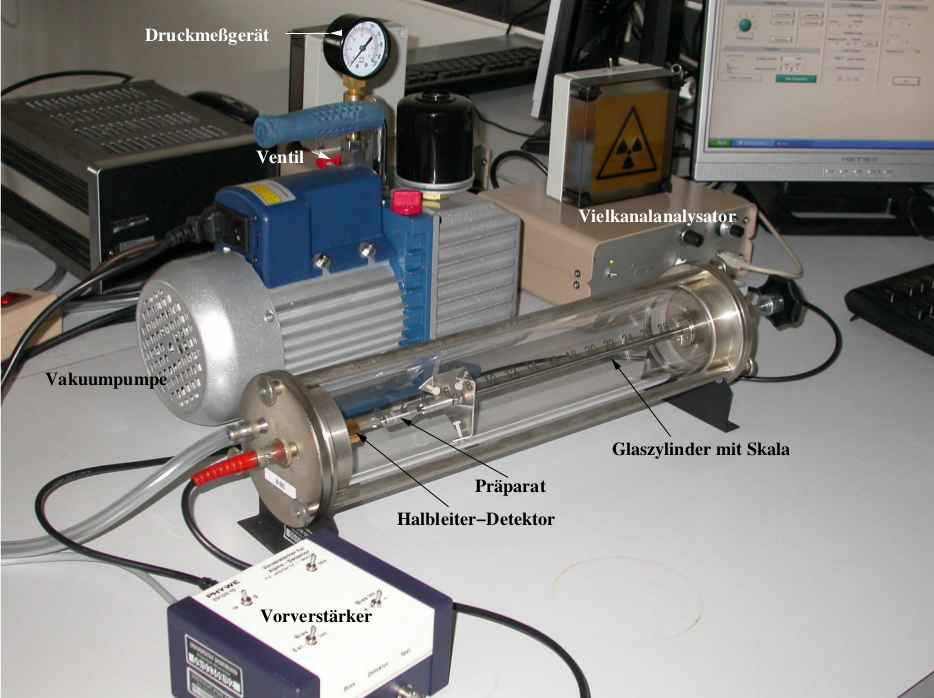
\includegraphics[height=7cm]{logos/Versuchsaufbau.png}
  \caption{Versuchsapparatur zur Bestimmung der Reichweite von \texorpdfstring{$\alpha$}{math}-Teilchen \cite{Anleitung}.}
  \label{fig:VB}
\end{figure}
\paragraph{Bestimmung der Reichweite von \texorpdfstring{$\alpha$}{math}-Teilchen}
\begin{itemize}
  \item Zuerst wird der Glaszylinder evakuiert und eine Position für das Präperat gewählt
  die während des ganzen Messprozesses konstant gehalten wird.
  \item Nun wird \SI{120}{\second} die Zählrate gemessen.
  \item Danach wird der Druck um \SI{50}{\bar} erhöht und gemessen.
  \item Die ersten drei Schritte werden so lange wiederhohlt bis ein merklicher
  Abfall der Zählrate zu beobachten ist. Dann sollte die Erhöhung der Drucks in
  kleineren Schritten erfolgen, so lange bis die Zählrate wieder konstant bleibt.
\end{itemize}
\paragraph{Statistik des radioaktiven Zerfalls}
Nun werden Position und Druck konstant gehalten. Dann wird 200 mal die
Zählrate über \SI{10}{\second} gemessen.
